\section{Jeffreys’ World: Probability as Belief}

To Harold Jeffreys, probability wasn’t just about coin flips or radioactive decay. It was about belief—how confident you are in a claim, and how that confidence should change as new evidence comes in.

This idea leads us straight into the heart of the Bayesian approach. Unlike Fisher, who avoided assigning probabilities to unknowns, Jeffreys leaned in. For him, even a parameter like \( \theta \)—say, the true probability of rain tomorrow—can have a probability distribution. It reflects what you believe, before and after you see the data.

Bayes’ theorem is the engine behind this approach:

\[
P(\theta \mid \text{data}) = \frac{P(\text{data} \mid \theta) P(\theta)}{P(\text{data})}
\]

In plain English:  
Start with what you believe (\( P(\theta) \)), update it based on the evidence (\( P(\text{data} \mid \theta) \)), and end up with a new belief (\( P(\theta \mid \text{data}) \)).


\begin{figure}[H]
\centering
\begin{tikzpicture}[scale=1.2, every node/.style={font=\small}]

  % Prior (top)
  \begin{scope}[yshift=7cm]
    \draw[->] (0,0) -- (3.5,0) node[right] {$\theta$};
    \draw[->] (0,0) -- (0,1.5) node[above] {$P(\theta)$};
    \draw[thick,blue,domain=0.2:3.2,smooth,variable=\x] 
      plot ({\x},{0.8*exp(-(\x-1.5)^2/0.5)});
    \node at (1.6,-0.4) {\textbf{Prior}};
  \end{scope}

  % Likelihood (middle)
  \begin{scope}[yshift=3.5cm]
    \draw[->] (0,0) -- (3.5,0) node[right] {$\theta$};
    \draw[->] (0,0) -- (0,1.5) node[above] {$P(\text{data} \mid \theta)$};
    \draw[thick,orange,domain=0.2:3.2,smooth,variable=\x] 
      plot ({\x},{exp(-(\x-2.2)^2/0.3)});
    \node at (1.6,-0.4) {\textbf{Likelihood}};
  \end{scope}

  % Posterior (bottom)
  \begin{scope}[yshift=0cm]
    \draw[->] (0,0) -- (3.5,0) node[right] {$\theta$};
    \draw[->] (0,0) -- (0,1.5) node[above] {$P(\theta \mid \text{data})$};
    \draw[thick,green!60!black,domain=0.2:3.2,smooth,variable=\x] 
      plot ({\x},{1.4*exp(-((\x-1.9)^2)/0.3)});
    \node at (1.6,-0.4) {\textbf{Posterior}};
  \end{scope}

  % Arrows connecting each step
  \draw[->, thick] (1.8,6.5) -- (1.8,5.1) node[midway, right] {\textbf{+ Data}};
  \draw[->, thick] (1.8,3.0) -- (1.8,1.6) node[midway, right] {\textbf{Bayes' Rule}};

  % Caption text
  \node[align=center] at (6,5.5) {
    \textbf{Bayesian Update:} \\ 
    Prior belief + evidence = posterior belief
  };

\end{tikzpicture}
\caption{In Jeffreys’ world, probability represents belief. Bayes’ theorem updates your belief about the parameter \( \theta \) as new data becomes available.}
\end{figure}


\begin{tcolorbox}[colback=gray!5!white, colframe=black!80!white, title={Historical Sidenote: From Bayes’s Theology to Jeffreys’s Science}]

  \textbf{Thomas Bayes} (1701–1761) was a Presbyterian minister and amateur mathematician whose posthumously published essay proposed a simple but revolutionary idea: that probability could express **degrees of belief**, not just frequencies of outcomes.
  
  Bayes framed his theorem in theological terms — attempting to defend divine providence by formalizing how rational belief should update in light of new evidence.
  
  \medskip
  
  Nearly two centuries later, \textbf{Harold Jeffreys} (1891–1989), a British physicist and philosopher of science, resurrected Bayes’s vision — but gave it a new philosophical backbone. For Jeffreys, probability was not just belief — it was **a logical extension of scientific reasoning**. He argued that inductive inference, done correctly, \textit{must} follow Bayesian logic.
  
  Where Bayes sought to justify faith, Jeffreys used the same mathematics to justify science.
  
  \medskip
  
  \textbf{Bayes made probability personal. Jeffreys made it principled.}
  
  \end{tcolorbox}
  


\subsubsection{Jeffreys’ Rule: What Should You Believe Before Seeing Anything?}

This leads to a natural question: if probability is belief, what should you believe when you know nothing at all?

Jeffreys tackled this with an elegant principle. He argued that your starting belief—your \textbf{prior}—should not favor one value over another just because of how it's labeled. If you rephrase the problem or change units, your beliefs should still make sense.

To do this, Jeffreys proposed a rule that builds your prior from the problem’s own geometry:

\[
\boxed{
P(\theta) \propto \sqrt{\mathcal{I}(\theta)}
}
\]

Here, \( \mathcal{I}(\theta) \) is the Fisher Information. Think of it like the "texture" of the problem: how much information the data carries about each possible value of \( \theta \). Jeffreys said: let the structure of the problem guide your uncertainty.


\begin{figure}[H]
\centering
\begin{tikzpicture}[scale=1.2, every node/.style={font=\small}]

  % Axes for Fisher Information
  \begin{scope}
    \draw[->] (0,0) -- (4.5,0) node[right] {$\theta$};
    \draw[->] (0,0) -- (0,2.2) node[above] {$\mathcal{I}(\theta)$};

    % Fisher Information curve: e.g., 1/θ^2 for illustration
    \draw[thick,blue,domain=0.3:4,smooth,variable=\x] 
      plot ({\x},{1/(\x)^2});

    \node[blue] at (3,1.6) {\( \mathcal{I}(\theta) \)};
    \node at (2,-0.5) {Fisher Information};
  \end{scope}

  % Arrow down
  \draw[->, thick] (2.3,0) -- (2.3,-0.8) node[midway, right] {\footnotesize Jeffreys’ Rule};

  % Axes for Prior
  \begin{scope}[yshift=-3cm]
    \draw[->] (0,0) -- (4.5,0) node[right] {$\theta$};
    \draw[->] (0,0) -- (0,2.2) node[above] {$P(\theta)$};

    % Jeffreys prior: sqrt of above (1/θ for illustration)
    \draw[thick,green!60!black,domain=0.3:4,smooth,variable=\x] 
      plot ({\x},{1/\x});

    \node[green!60!black] at (3,1.6) {\( P(\theta) \propto \sqrt{\mathcal{I}(\theta)} \)};
    \node at (2,-0.5) {Jeffreys Prior};
  \end{scope}

  % Title
  \node[align=center] at (6.5,1.5) {
    \textbf{Jeffreys’ Rule:} \\ 
    Let the geometry of the model (Fisher Information) guide your prior
  };

\end{tikzpicture}
\caption{Jeffreys’ Rule: Your prior belief should reflect the information structure of the problem. Use \( P(\theta) \propto \sqrt{\mathcal{I}(\theta)} \) to build invariant, objective priors.}
\end{figure}


\subsubsection{Why a Flat Prior Isn’t Always Fair}

Imagine you’re trying to guess the true probability of heads for a coin, and you say: “Let’s just assign equal probability to every possible value between 0 and 1.” Sounds fair, right?

But now imagine instead of working with \( \theta \), you switch to the log-odds: \( \phi = \log(\theta / (1 - \theta)) \). Suddenly, that “flat” prior in \( \theta \) becomes distorted in \( \phi \). You didn’t change the problem—just how you described it—but your beliefs got skewed.

Jeffreys’ prior avoids this. It adjusts automatically no matter how you rephrase or reparameterize the problem. It doesn’t just look fair—it \textit{stays} fair, in any coordinate system.


\begin{figure}[H]
\centering
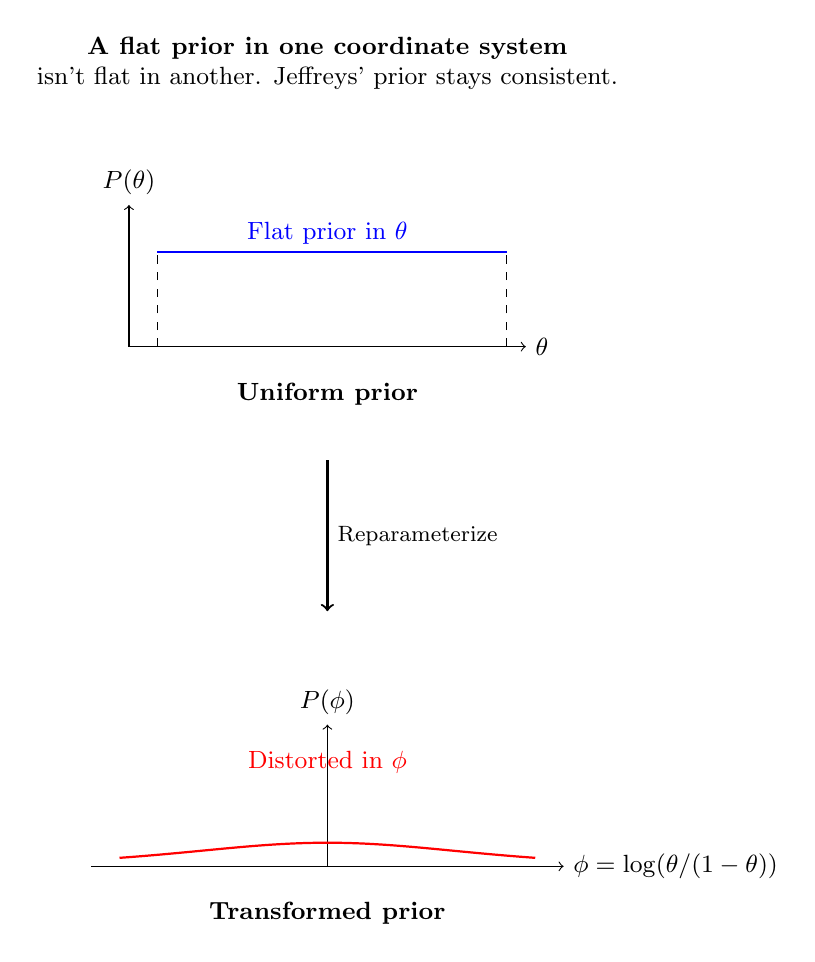
\begin{tikzpicture}[scale=1.2, every node/.style={font=\small}]

  % Annotation above the first plot
  \node[align=center] at (2.1,8.5) {
    \textbf{A flat prior in one coordinate system} \\
    isn’t flat in another. Jeffreys’ prior stays consistent.
  };

  % Top plot: flat prior in θ-space
  \begin{scope}[yshift=5.5cm]
    \draw[->] (0,0) -- (4.2,0) node[right] {$\theta$};
    \draw[->] (0,0) -- (0,1.5) node[above] {$P(\theta)$};

    % Flat prior
    \draw[thick,blue] (0.3,1) -- (4,1);
    \draw[dashed] (0.3,0) -- (0.3,1);
    \draw[dashed] (4,0) -- (4,1);

    \node[blue] at (2.1,1.2) {Flat prior in \( \theta \)};
    \node at (2.1,-0.5) {\textbf{Uniform prior}};
  \end{scope}

  % Arrow to transformed space
  \draw[->, thick] (2.1,4.3) -- (2.1,2.7) node[midway, right] {\footnotesize Reparameterize};

  % Bottom plot: transformed prior in φ-space
  \begin{scope}[yshift=0cm, xshift=0cm]
    \draw[->] (-2.5+2.1,0) -- (2.5+2.1,0) node[right] {$\phi = \log(\theta / (1 - \theta))$};
    \draw[->] (2.1,0) -- (2.1,1.5) node[above] {$P(\phi)$};

    % Distorted transformed prior (bell-shaped)
    \draw[thick,red,domain=-2.2:2.2,smooth,variable=\x] 
      plot ({\x + 2.1},{1/(exp(\x)+exp(-\x)+2)});

    \node[red] at (2.1,1.1) {Distorted in \( \phi \)};
    \node at (2.1,-0.5) {\textbf{Transformed prior}};
  \end{scope}

\end{tikzpicture}
\caption{Flat priors can be misleading under reparameterization. While the prior on \( \theta \) may appear fair, its transformed version in \( \phi = \log(\theta / (1 - \theta)) \) becomes skewed. Jeffreys’ prior avoids this by adapting to the geometry of the problem.}
\end{figure}




\subsubsection{Example: Flipping Coins}

Say you’re modeling a series of coin flips, trying to guess the true probability \( \theta \) of landing heads.

Jeffreys' prior for this setup is:

\[
P(\theta) \propto \frac{1}{\sqrt{\theta(1 - \theta)}}
\]

This prior leans slightly toward extreme values (near 0 or 1), because in those regions, data is more informative. A coin that lands heads almost every time gives clearer signals than one that’s 50-50. Jeffreys' prior reflects that.


\begin{figure}[H]
\centering
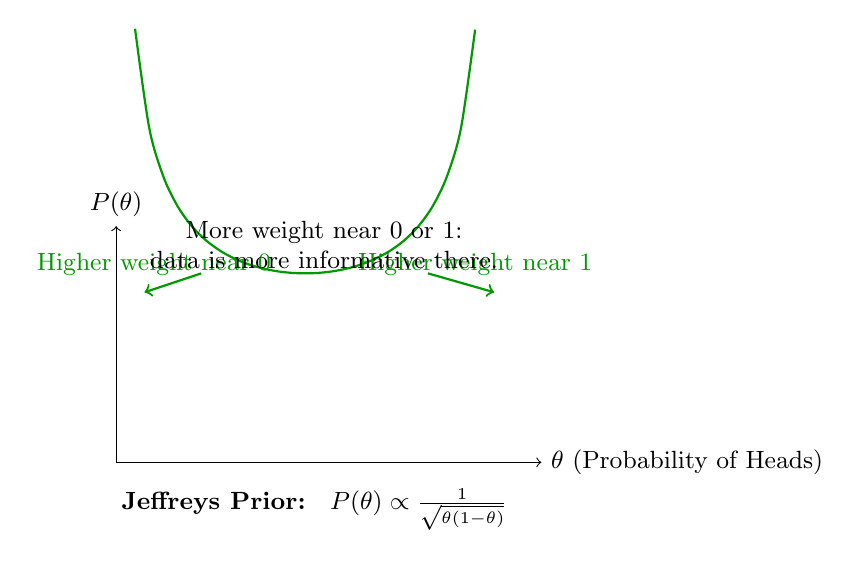
\begin{tikzpicture}[scale=1.2, every node/.style={font=\small}]

  % Axes
  \draw[->] (0,0) -- (4.5,0) node[right] {$\theta$ (Probability of Heads)};
  \draw[->] (0,0) -- (0,2.5) node[above] {$P(\theta)$};

  % Jeffreys prior curve
  \draw[thick,green!60!black,domain=0.05:0.95,smooth,variable=\t] 
    plot ({\t*4}, {1/sqrt(\t*(1-\t))});

  % Labels near extremes
  \node[green!60!black] at (0.4,2.1) {Higher weight near 0};
  \node[green!60!black] at (3.8,2.1) {Higher weight near 1};
  \draw[->, thick, green!60!black] (0.9,2.0) -- (0.3,1.8);
  \draw[->, thick, green!60!black] (3.3,2.0) -- (4,1.8);

  % Center annotation
  \node at (2.1,-0.5) {\textbf{Jeffreys Prior: } \( P(\theta) \propto \frac{1}{\sqrt{\theta(1 - \theta)}} \)};

  % Intuition note
  \node[align=center] at (2.2,2.3) {
    More weight near 0 or 1: \\
    data is more informative there.
  };

\end{tikzpicture}
\caption{Jeffreys' prior for coin flips leans toward extreme values of \( \theta \), reflecting that a coin biased toward heads or tails yields more informative data than a perfectly fair coin.}
\end{figure}






\subsubsection{Example: Measuring a Scale}

Now imagine you're estimating something like a standard deviation \( \sigma \)—how spread out the data is. Should your prior believe that \( \sigma = 1 \) is just as likely as \( \sigma = 1000 \)? What about \( \sigma = 0.001 \)?

Jeffreys' prior here is:

\[
P(\sigma) \propto \frac{1}{\sigma}
\]

This is called a log-uniform prior. It doesn’t favor any specific scale—it gives equal weight to each order of magnitude. Whether you’re measuring bacteria or galaxies, your belief starts out scale-invariant.

\begin{figure}[H]
\centering
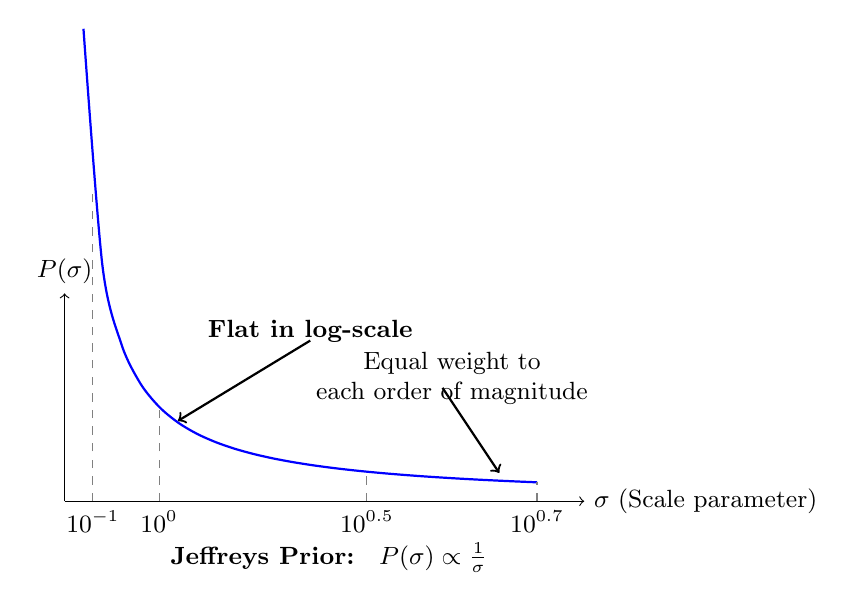
\begin{tikzpicture}[scale=1.2, every node/.style={font=\small}]

  % Axes for sigma space
  \draw[->] (0,0) -- (5.5,0) node[right] {$\sigma$ (Scale parameter)};
  \draw[->] (0,0) -- (0,2.2) node[above] {$P(\sigma)$};

  % Plot 1/sigma
  \draw[thick,blue,domain=0.2:5,smooth,variable=\s] 
    plot ({\s}, {1/\s});

  % Dashed lines to mark orders of magnitude
  \foreach \x/\label in {0.3/{10^{-1}}, 1/{10^{0}}, 3.2/{10^{0.5}}, 5/{10^{0.7}}} {
    \draw[dashed,gray] (\x,0) -- (\x,{1/\x});
    \node[below] at (\x,0) {\( \label \)};
  }

  % Annotation: flat in log-space
  \node at (2.6,1.8) {\textbf{Flat in log-scale}};
  \draw[->, thick] (2.6,1.7) -- (1.2,0.85);

  % Label for prior
  \node at (2.8,-0.6) {\textbf{Jeffreys Prior: } \( P(\sigma) \propto \frac{1}{\sigma} \)};

  % Extra annotation
  \node[align=center] at (4.1,1.3) {
    Equal weight to\\ each order of magnitude
  };
  \draw[->, thick] (4,1.2) -- (4.6,0.3);

\end{tikzpicture}
\caption{Jeffreys’ prior for scale parameters like \( \sigma \) gives equal belief to every order of magnitude. It's invariant to rescaling—useful whether you're measuring atoms or galaxies.}
\end{figure}







\subsubsection{Jeffreys’ Legacy: Let the Problem Speak}

Jeffreys’ big insight was this:

\begin{quote}
If you're going to assign beliefs, start by respecting the structure of the problem. Let the math guide your uncertainty.
\end{quote}

His rule doesn’t come from intuition or convenience—it comes from symmetry, geometry, and fairness. It’s not perfect: sometimes it’s mathematically messy, and it doesn’t incorporate prior knowledge when you \textit{do} have some. But when you're starting from scratch and want to be principled, Jeffreys offers a powerful compass.









\subsection{The Monty Hall Problem (Now with a Million Doors)}

Let’s play a game.

You’re standing in front of \textbf{one million doors}. Behind one of them is a shiny new car. Behind the rest? Goats. Fluffy, bleating, disappointingly non-motorized goats.

You pick one door—say, Door \#17. You’re hopeful. Maybe lucky.

Then the host, who knows exactly where the car is, starts opening doors. One after another, goats. He opens \textbf{999,998 of them}. Now only two doors remain unopened: the one you picked, and one other.

Then he turns to you and says:  
\textit{“Want to stick with your original door, or switch to the other one?”}

\vspace{0.5em}
\noindent
\textbf{At this point, most people hesitate.}  
“There are two doors left,” they think. “It’s a coin flip now, right?”

\textbf{Actually... no. Not even close.}

\vspace{0.5em}
\noindent
Let’s rewind. When you first picked a door, your chances of choosing the car were 1 in a million. That’s about as close to zero as you can get. That means the car was almost certainly \textit{not} behind your door.

But then the host—who knows exactly where the car is—opens every other door except one. And he makes sure those opened doors all reveal goats. He’s not just randomly flipping doors open. He’s carefully steering the game so that one other door stays shut.

All of the original “almost certainly not your door” probability—999,999 chances out of a million—gets funneled onto that one remaining unopened door. The odds haven’t reset. The host didn’t flip a coin. He revealed information. And that changed what you should believe.

\textbf{You should switch. The odds are 999,999 to 1 in your favor.}

\vspace{1em}
\noindent
\textbf{What does this have to do with statistics? Everything.}




\begin{figure}[H]
\centering
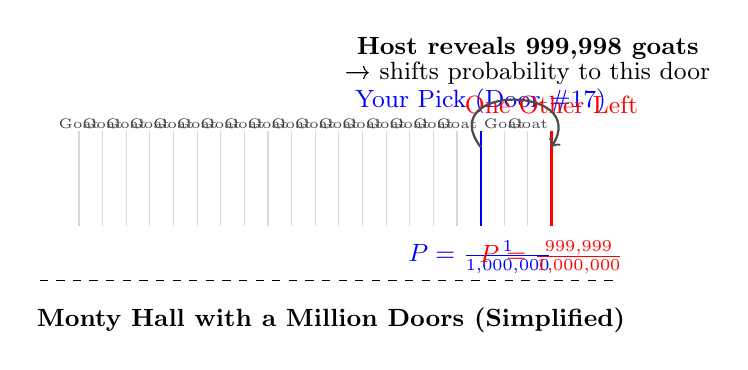
\begin{tikzpicture}[scale=1, every node/.style={font=\small}]

  % Represent doors with short vertical lines
  \foreach \i in {0,1,...,19} {
    \draw[gray!60] (\i*0.3,0) --++ (0,1.2);
  }

  % Highlight Door #17 (user's pick)
  \draw[thick,blue] (5.1,0) --++ (0,1.2);
  \node[blue,above] at (5.1,1.3) {Your Pick (Door \#17)};
  \node[blue] at (5.1,-0.4) {\(P = \frac{1}{1{,}000{,}000}\)};

  % Highlight the only other unopened door
  \draw[thick,red] (6.0,0) --++ (0,1.2);
  \node[red,above] at (6.0,1.3) {One Other Left};
  \node[red] at (6.0,-0.4) {\(P = \frac{999{,}999}{1{,}000{,}000}\)};

  % Draw opened goat doors (symbolic)
  \foreach \i in {0,1,...,16,18,19} {
    \draw[gray!30] (\i*0.3,0) --++ (0,1.2);
    \node[gray!50!black] at (\i*0.3,1.3) {\tiny Goat};
  }

  % Arrow showing probability shift
  \draw[->, thick,gray!60!black] (5.1,1.0) .. controls (4.5,1.8) and (6.5,1.8) .. (6.0,1.0);
  \node[align=center] at (5.7,2.1) {
    \textbf{Host reveals 999,998 goats} \\[-2pt]
    → shifts probability to this door
  };

  % Optional visual separator
  \draw[dashed] (-0.5,-0.7) -- (6.8,-0.7);
  \node at (3.2,-1.2) {\textbf{Monty Hall with a Million Doors (Simplified)}};

\end{tikzpicture}
\caption{In the Monty Hall problem with a million doors, your first pick had a 1-in-a-million chance of being correct. After the host reveals 999,998 goats, all remaining probability shifts to the last unopened door. You should switch.}
\end{figure}





\paragraph{Fisher’s View: Fixed Reality, No Beliefs}

Ronald Fisher wouldn’t call this a probability puzzle at all. To him, the car isn’t in a quantum superposition—it’s already behind one specific door. Reality is fixed. There’s no uncertainty in the world itself, only in your limited access to it. You either picked the correct door or you didn’t. End of story.

In Fisher’s world, probability isn’t about what you believe or how confident you feel. It’s not a measure of personal doubt. Instead, it’s a tool for describing what would happen if you repeated the experiment many, many times—an abstraction of long-run behavior. Flip a million coins. Run a million Monty Hall games. Analyze the frequencies. That’s where probability lives.

What about the host’s actions? For Fisher, those are data. You use them to condition your model, not to update a belief. There’s no “Bayesian update” here—just inference based on the sample space of possible outcomes. Fisher would say: forget belief. Stick to models, data, and likelihoods.



\begin{figure}[H]
\centering
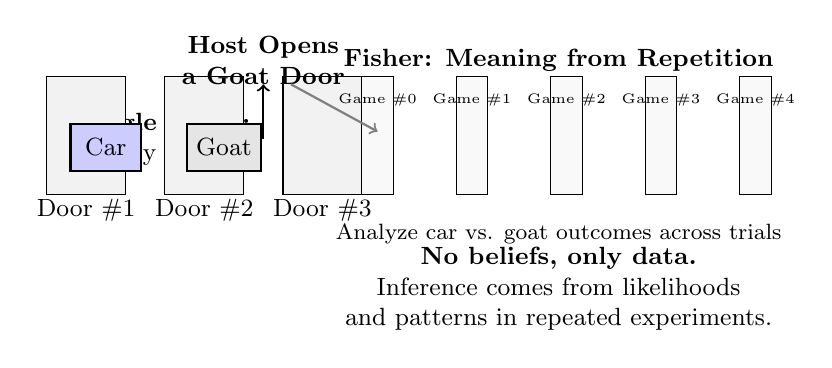
\begin{tikzpicture}[scale=1, every node/.style={font=\small}]

  % Row of doors - single game
  \node[align=center] at (1.5,3.2) {\textbf{Single Game:}\\Reality is Fixed};

  \foreach \i in {0,1,2} {
    \draw[fill=gray!10] (\i*1.5,2.5) rectangle ++(1,1.5);
    \node at (\i*1.5+0.5,2.3) {Door \#\the\numexpr\i+1\relax};
  }

  % Car behind Door #1
  \node[draw, thick, fill=blue!20, minimum width=0.9cm, minimum height=0.6cm] at (0.75,3.1) {Car};

  % Goat behind Door #3
  \node[draw, thick, fill=gray!20, minimum width=0.9cm, minimum height=0.6cm] at (2.25,3.1) {Goat};

  % Host's action annotation
  \draw[->, thick] (2.75,3.2) -- (2.75,3.9);
  \node[align=center] at (2.75,4.2) {\textbf{Host Opens} \\ \textbf{a Goat Door}};

  % Repeated trials section
  \node[align=center] at (6.5,4.2) {\textbf{Fisher: Meaning from Repetition}};

  \foreach \x in {0,...,4} {
    \draw[fill=gray!5] (4+\x*1.2,2.5) rectangle ++(0.4,1.5);
    \node at (4+\x*1.2+0.2,3.7) {\tiny Game \#\x};
  }

  % Frequencies label
  \node at (6.5,2) {\footnotesize Analyze car vs. goat outcomes across trials};

  % Arrow from host action to repeated trials
  \draw[->, thick, gray] (3.1,3.9) -- (4.2,3.3);

  % Summary annotation
  \node[align=center] at (6.5,1.3) {
    \textbf{No beliefs, only data.} \\
    Inference comes from likelihoods \\
    and patterns in repeated experiments.
  };

\end{tikzpicture}
\caption{Fisher’s view: The car is behind a specific door. The host’s action is data, not belief-shifting evidence. Probability describes the long-run behavior of repeatable processes—not subjective uncertainty.}
\end{figure}






\paragraph{Jeffreys’ View: Uncertainty Is the Whole Game}

Harold Jeffreys would take a very different view. When you picked Door \#17, you weren’t uncovering a truth—you were expressing a belief. The car was somewhere, yes, but your knowledge of where was deeply uncertain. Your initial belief that you had chosen correctly was 1 in a million. And crucially, that was your belief—not because of metaphysics, but because of the information you had.

Then something important happened: the host acted. He didn’t just open doors at random—he used privileged information to show you 999,998 goats. He shaped the evidence. And in the Bayesian world Jeffreys championed, evidence is everything. When new data appears, your belief should shift. That’s the whole point.

Jeffreys wouldn’t say, “Now it’s a 50/50 chance.” He’d say: the host’s actions are part of the data. They tell a story, and that story overwhelmingly supports the hypothesis that the other unopened door is the right one. Probability isn’t a fixed feature of the universe—it’s a reflection of what you know, and how honestly you update that knowledge when the world gives you more to go on.

\begin{quote}
``The world didn’t change. But what you know about it did. And probability is about what you know.''
\end{quote}



\begin{figure}[H]
\centering
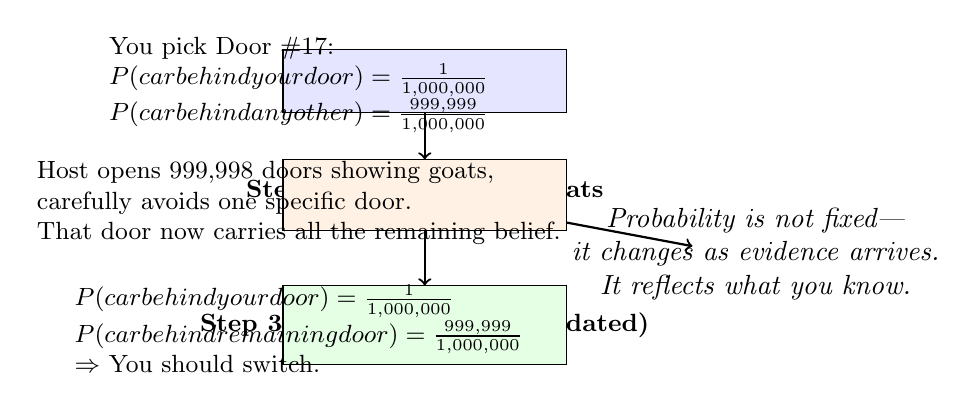
\begin{tikzpicture}[scale=1, every node/.style={font=\small}]

  % Step 1: Prior belief
  \node[align=center] at (1.8,4.3) {\textbf{Step 1: Prior Belief}};

  \draw[fill=blue!10] (0,3.8) rectangle ++(3.6,0.8);
  \node[align=left] at (0.2,4.15) {
    You pick Door \#17: \\ 
    \(P(\text{car behind your door}) = \frac{1}{1{,}000{,}000}\)\\
    \(P(\text{car behind any other}) = \frac{999{,}999}{1{,}000{,}000}\)
  };

  % Step 2: Host reveals doors
  \node[align=center] at (1.8,2.8) {\textbf{Step 2: Host Reveals Goats}};

  \draw[fill=orange!10] (0,2.3) rectangle ++(3.6,0.9);
  \node[align=left] at (0.2,2.65) {
    Host opens 999,998 doors showing goats, \\ 
    carefully avoids one specific door. \\
    That door now carries all the remaining belief.
  };

  % Step 3: Posterior belief
  \node[align=center] at (1.8,1.1) {\textbf{Step 3: Posterior Belief (Updated)}};

  \draw[fill=green!10] (0,0.6) rectangle ++(3.6,1.0);
  \node[align=left] at (0.2,1.05) {
    \(P(\text{car behind your door}) = \frac{1}{1{,}000{,}000}\) \\
    \(P(\text{car behind remaining door}) = \frac{999{,}999}{1{,}000{,}000}\) \\
    $\Rightarrow$ You should switch.
  };

  % Arrows between steps
  \draw[->, thick] (1.8,3.8) -- (1.8,3.2);
  \draw[->, thick] (1.8,2.3) -- (1.8,1.6);

  % Belief emphasis
  \node[align=center, font=\itshape] at (6,2) {
    Probability is not fixed— \\
    it changes as evidence arrives. \\
    It reflects what you know.
  };

  \draw[thick, ->] (3.6,2.4) -- (5.2,2.1);

\end{tikzpicture}
\caption{Jeffreys’ view: Probability reflects what you know. As the host reveals goats, you should update your beliefs. The final unopened door now carries almost all the probability.}
\end{figure}




\paragraph{Why This Isn’t Just a Game Show Trick}

This strange little scenario—just you, a million doors, and one very smug host—turns out to touch one of the deepest philosophical divides in statistics:

\begin{itemize}
    \item \textbf{Frequentist view:} Probability is about long-run frequencies and fixed truths. The car is somewhere, and your job is to make sense of repeated patterns over many hypothetical games.
    \item \textbf{Bayesian view:} Probability is about uncertainty. It’s about how you reason under partial knowledge, and how your beliefs should evolve when new information comes in.
\end{itemize}

In everyday life, we’re almost always Bayesians. When your GPS says there’s a traffic jam ahead, you reroute. When a friend cancels lunch twice in a row, your estimate of whether they’re flaking goes up. We learn. We revise. We update. That’s what belief is for.

But in statistics—and especially in machine learning—this philosophical fork in the road becomes a modeling choice with consequences. Are model parameters fixed but unknown quantities you estimate, like in Fisher’s world? Or are they uncertain values with distributions you refine as new data arrives, as Jeffreys would have it?

The Monty Hall problem—with a million doors—makes that difference hard to ignore. You should switch. Not because the car magically moved, but because the host's actions revealed something. Not because the odds reset, but because your understanding changed.

And that’s what statistics, at its best, is all about: learning from the world, one update at a time.









\subsection{Confidence vs. Credible Intervals: A Tale of Two Interpretations}

Let’s say you’re running a clinical trial for a new drug. After crunching the numbers, you find that it seems to lower blood pressure by 3 units. But this is science, not science fiction—you’re never 100\% sure. So you report your result like this:

\[
[1.8,\ 4.2]
\]

But what does this interval really mean?

\begin{itemize}
    \item \textbf{Frequentist (Confidence Interval):}  
    “If we ran this experiment a zillion times, 95\% of those intervals would contain the true effect.”
    
    \item \textbf{Bayesian (Credible Interval):}  
    “Given this data, there’s a 95\% chance the true effect is between 1.8 and 4.2.”
\end{itemize}

They sound similar. But they come from completely different worldviews.

The frequentist treats the effect size as a fixed number—unknown, yes, but not random. The randomness lives in the data. So confidence intervals are about long-run performance: how well the method does across infinite repetitions of the experiment. It’s not about *this* interval, or *this* dataset—it’s about the procedure. You're not allowed to say there's a 95\% chance the true value lies in this interval. That's not how frequentist probability works.

The Bayesian, by contrast, is comfortable treating the effect as uncertain. It’s not some metaphysical constant hiding behind the curtain—it’s a quantity we don’t fully know yet. So the Bayesian says: “Here’s what we believe about the effect, based on what we’ve seen.” The credible interval is a direct statement about the probability that the true value lies within the reported range. It’s a statement about this specific analysis, not an imagined universe of infinite trials.

The difference may seem subtle, even academic. But in practice, it can change how you make decisions, interpret findings, and communicate results. One tells you how your method behaves in the long run. The other tells you what you should believe, right now, given what you know.

And depending on the stakes—say, recommending a drug to millions of people—that distinction suddenly matters a lot.




\begin{figure}[H]
\centering
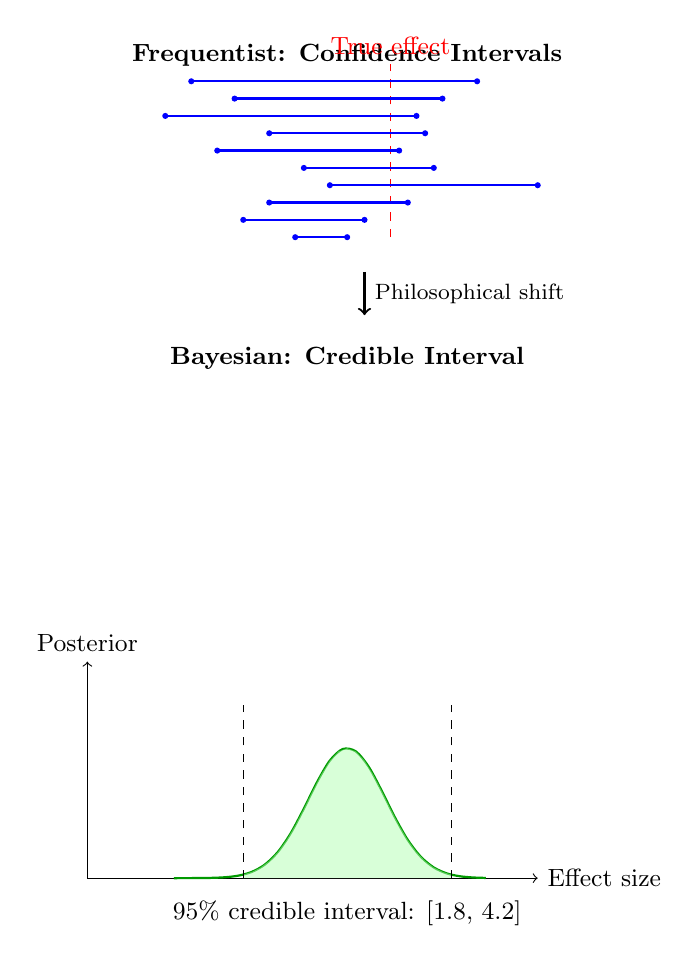
\begin{tikzpicture}[scale=1.1, every node/.style={font=\small}]

  % Top: Frequentist confidence intervals
  \node at (3,10.5) {\textbf{Frequentist: Confidence Intervals}};

  % True effect (vertical line)
  \draw[dashed,red] (3.5,8.4) -- (3.5,10.4);
  \node[red,above] at (3.5,10.4) {True effect};

  % Intervals (shifted to match vertical layout)
  \foreach \y/\xlow/\xhigh/\hit in {
    10.2/1.2/4.5/yes,
    10.0/1.7/4.1/yes,
    9.8/0.9/3.8/yes,
    9.6/2.1/3.9/yes,
    9.4/1.5/3.6/yes,
    9.2/2.5/4.0/yes,
    9.0/2.8/5.2/yes,
    8.8/2.1/3.7/yes,
    8.6/1.8/3.2/yes,
    8.4/2.4/3.0/no
  } {
    \ifthenelse{\equal{\hit}{yes}}{
      \draw[blue,thick] (\xlow,\y) -- (\xhigh,\y);
    }{
      \draw[blue,thick,dashed] (\xlow,\y) -- (\xhigh,\y);
    }
    \fill[blue] (\xlow,\y) circle (1pt);
    \fill[blue] (\xhigh,\y) circle (1pt);
  }

  % Arrow connecting to next panel
  \draw[->,thick] (3.2,8.0) -- (3.2,7.5) node[midway, right] {\footnotesize Philosophical shift};

  % Bottom: Bayesian posterior and credible interval
  \begin{scope}[yshift=0cm]
    \node at (3,7) {\textbf{Bayesian: Credible Interval}};
    
    % Axes
    \draw[->] (0,1.0) -- (5.2,1.0) node[right] {Effect size};
    \draw[->] (0,1.0) -- (0,3.5) node[above] {Posterior};

    % Posterior curve
    \draw[thick,green!60!black,domain=1:4.6,smooth,variable=\x] 
      plot ({\x},{1.0 + 1.5*exp(-((\x - 3)^2)/0.4)});

    % Credible interval shaded
    \fill[green!30,opacity=0.5] (1.8,1.0) -- plot[domain=1.8:4.2] ({\x},{1.0 + 1.5*exp(-((\x - 3)^2)/0.4)}) -- (4.2,1.0) -- cycle;

    % Interval ends
    \draw[dashed] (1.8,1.0) -- (1.8,3.0);
    \draw[dashed] (4.2,1.0) -- (4.2,3.0);
    \node at (3,0.6) {95\% credible interval: [1.8,\ 4.2]};
  \end{scope}

\end{tikzpicture}
\caption{Frequentist confidence intervals succeed in the long run—most contain the true effect (a fixed, unknown value). Bayesian credible intervals express belief about the parameter given the data. Both give you an interval, but the interpretation is fundamentally different.}
\end{figure}






\paragraph{The Frequentist View: It’s Not About This Trial}

In the frequentist world, the true effect is a fixed number—a constant of nature. You don’t know what it is, but it’s out there, unchanging. Once you run your experiment and collect your data, the interval you compute is fixed too. It either contains the truth or it doesn’t. There’s no more randomness left to reason about.

So what can you say?  
You can say this: “If we repeated this exact experiment an infinite number of times, using the same method to construct intervals each time, then 95\% of those intervals would contain the true effect.” That’s the meaning of a 95\% confidence interval.

But here’s the catch: this doesn’t tell you anything about the specific interval you just calculated. You’re not allowed to say there’s a 95\% chance the true value lies inside it. From a frequentist perspective, that would be a category error—there’s no probability involved once the data are in. Either the interval captured the truth, or it didn’t. You just don’t know which.

It’s like saying: “My archery technique is good—I hit the target 95\% of the time.” That’s about your performance over many shots. But when you shoot a single arrow and it’s buried in the hay, you can’t say there's a 95\% chance it hit the bullseye. Either it did or it didn’t. The only thing that has a probability is the process, not the outcome.

This philosophy prioritizes rigor, objectivity, and repeatability. But it can feel oddly hands-off when making decisions in the moment. After all, when a doctor reads your interval, they don’t care about long-run coverage—they care about what’s likely to be true *now*.


\begin{figure}[H]
\centering
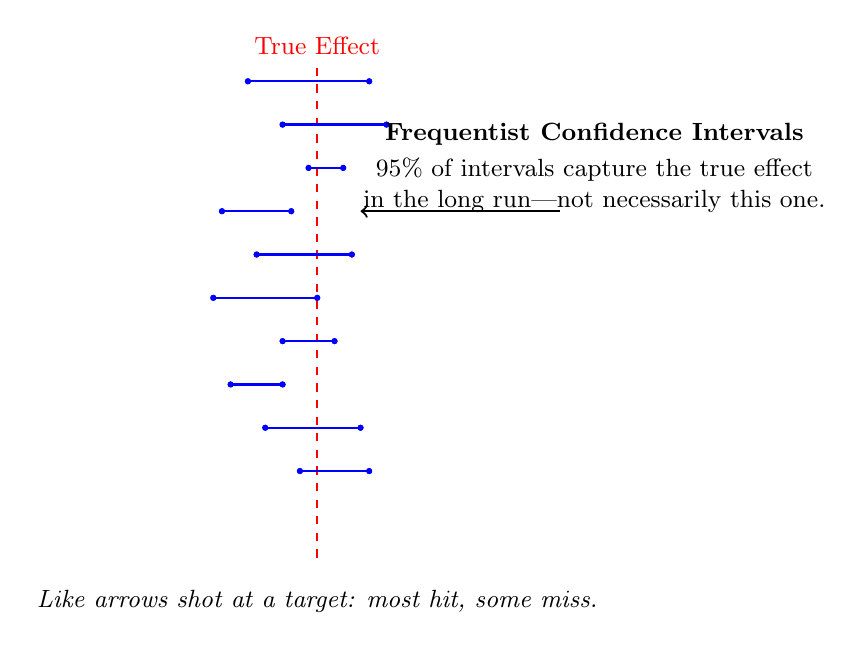
\begin{tikzpicture}[scale=1.1, every node/.style={font=\small}]

  % Vertical line: the fixed true effect
  \draw[dashed,red,thick] (4,0) -- (4,5.7);
  \node[red,above] at (4,5.7) {True Effect};

  % Draw 10 confidence intervals (most contain the truth)
  \foreach \y/\left/\right/\hit in {
    5.5/3.2/4.6/yes,
    5.0/3.6/4.8/yes,
    4.5/3.9/4.3/yes,
    4.0/2.9/3.7/no,
    3.5/3.3/4.4/yes,
    3.0/2.8/4.0/yes,
    2.5/3.6/4.2/yes,
    2.0/3.0/3.6/no,
    1.5/3.4/4.5/yes,
    1.0/3.8/4.6/yes
  } {
    \ifthenelse{\equal{\hit}{yes}}{
      \draw[blue,thick] (\left,\y) -- (\right,\y);
      \fill[blue] (\left,\y) circle (1pt);
      \fill[blue] (\right,\y) circle (1pt);
    }{
      \draw[blue,dashed,thick] (\left,\y) -- (\right,\y);
      \fill[blue] (\left,\y) circle (1pt);
      \fill[blue] (\right,\y) circle (1pt);
    }
  }

  % Caption text
  \node[align=center] at (7.2,4.5) {
    \textbf{Frequentist Confidence Intervals} \\[2pt]
    95\% of intervals capture the true effect \\ 
    in the long run—not necessarily this one.
  };

  % Arrow to highlight the idea of long-run interpretation
  \draw[->,thick] (6.8,4.0) -- (4.5,4.0);

  % Optional metaphor label
  \node at (4,-0.5) {\textit{Like arrows shot at a target: most hit, some miss.}};

\end{tikzpicture}
\caption{In the frequentist view, confidence intervals are about the long-run performance of a method—not about any specific interval. Each one either contains the true value or it doesn’t, and there’s no probability attached after the data are in.}
\end{figure}






\paragraph{The Bayesian View: What Do You Believe Now?}

Bayesians think differently. For them, the data isn’t random—it already happened. What’s uncertain is the parameter you’re trying to estimate: the true effect size, the chance of rain tomorrow, the odds your friend is telling the truth. So you model that uncertainty directly, using probability distributions to represent what you believe about the world.

This belief isn’t made up out of thin air. You start with a prior: what you believed before seeing the data. Then you apply Bayes’ rule to update those beliefs using the evidence in front of you. The result is a posterior distribution—a full picture of what you now think is plausible.

From this distribution, you can extract a credible interval: a range that contains, say, 95\% of your updated beliefs. Unlike a frequentist confidence interval, this one is about your current state of knowledge. It’s perfectly valid to say:  
\begin{quote}
“There’s a 95\% chance the true effect lies between 1.8 and 4.2.”  
\end{quote}

That’s not just a statistical artifact—it’s a statement about what you believe, given what you’ve seen. In this worldview, probability isn’t about what happens in the long run. It’s about what you know right now, and how confidently you know it.

\paragraph{A Quick Detour Back to Monty Hall}

Remember the million-door game show?

You picked Door \#17. The host—who knows where the car is—opened 999,998 doors to reveal goats, leaving only yours and one other unopened door.

A frequentist might hesitate. “Sure,” they’d say, “this seems suspicious. But we can’t draw firm conclusions from just one game. Let’s rerun the experiment thousands of times, then compute how often switching wins.”

But the Bayesian doesn’t wait for reruns. They’ve already seen enough.

“The host’s actions weren’t random,” they’d say. “They were deliberate and informative. Given that, I now assign almost all my belief—about 99.9999\% of it—to the remaining unopened door. Switching isn’t just a good bet—it’s a no-brainer.”

It’s the same situation, the same data. But the philosophical difference is stark.

The frequentist sees data as a sample from a larger process. The Bayesian sees it as evidence to be interpreted now. One says: “Let’s study this over the long haul.” The other says: “What do I believe, right here, in this moment?”

And depending on the context—clinical trials, weather forecasts, policy decisions—that shift in mindset can change everything.


\begin{figure}[H]
\centering
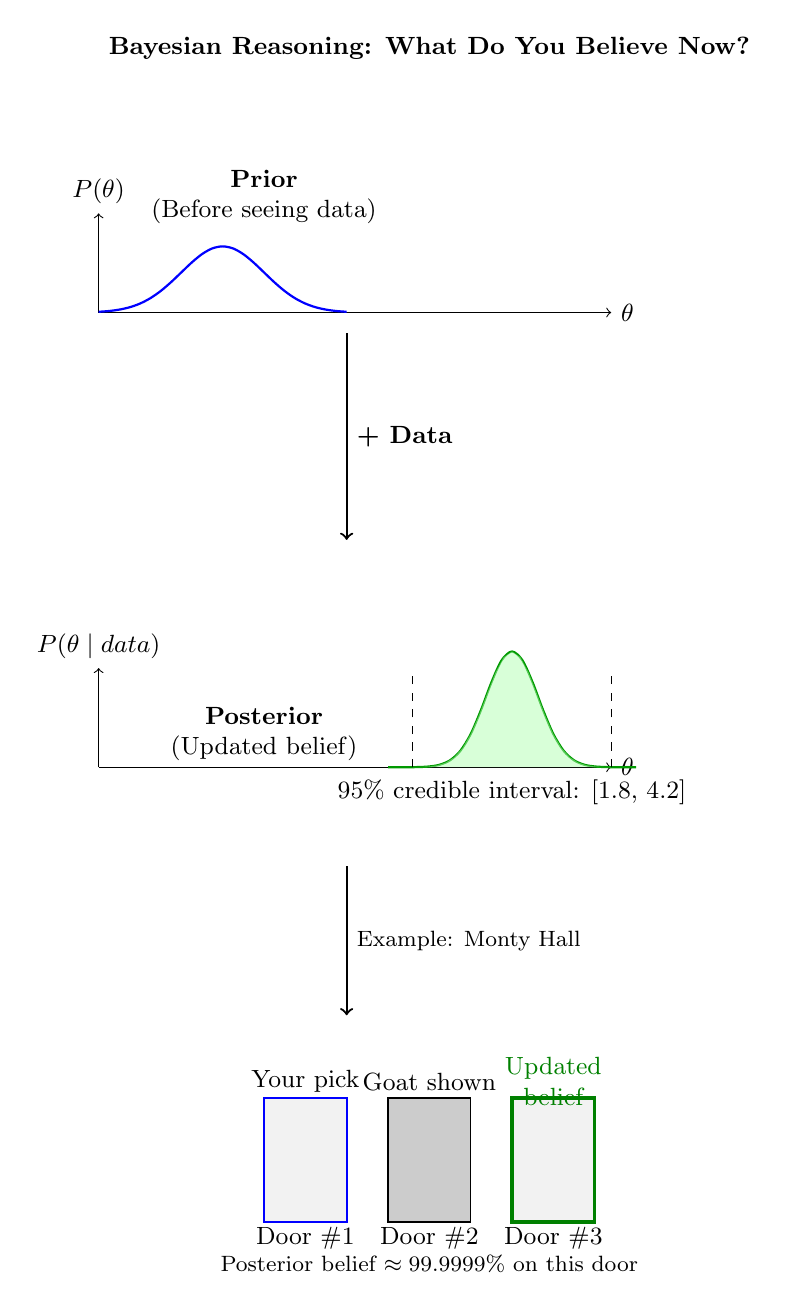
\begin{tikzpicture}[scale=1.05, every node/.style={font=\small}]

  % ========================
  % Title
  \node at (4,18.2) {\textbf{Bayesian Reasoning: What Do You Believe Now?}};
  % ========================

  % ========================
  % PRIOR PANEL
  \begin{scope}[yshift=0cm] % Adjust yshift to move prior block
    \node[align=center] at (2,16.4) {\textbf{Prior} \\ (Before seeing data)};
    \draw[->] (0,15) -- (6.2,15) node[right] {$\theta$};
    \draw[->] (0,15) -- (0,16.2) node[above] {$P(\theta)$};
    \draw[thick,blue,domain=0:3,smooth,variable=\x] 
      plot ({\x}, {15 + 0.8*exp(-((\x - 1.5)^2)/0.5)});
  \end{scope}
  % ========================

  % Arrow between Prior and Posterior
  \draw[->, thick] (3,14.75) -- (3,12.25) node[midway, right] {\textbf{+ Data}};

  % ========================
  % POSTERIOR PANEL
  \begin{scope}[yshift=-2.5cm] % Adjust yshift to move posterior block
    \node[align=center] at (2,12.4) {\textbf{Posterior} \\ (Updated belief)};
    \draw[->] (0,12) -- (6.2,12) node[right] {$\theta$};
    \draw[->] (0,12) -- (0,13.2) node[above] {$P(\theta \mid \text{data})$};
    \draw[thick,green!60!black,domain=3.5:6.5,smooth,variable=\x] 
      plot ({\x}, {12 + 1.4*exp(-((\x - 5)^2)/0.2)});

    % Credible interval
    \fill[green!30,opacity=0.5] (3.8,12) -- plot[domain=3.8:6.2] 
      ({\x}, {12 + 1.4*exp(-((\x - 5)^2)/0.2)}) -- (6.2,12) -- cycle;
    \draw[dashed] (3.8,12) -- (3.8,13.1);
    \draw[dashed] (6.2,12) -- (6.2,13.1);
    \node at (5,11.7) {95\% credible interval: [1.8,\ 4.2]};
  \end{scope}
  % ========================

  % Arrow to Monty Hall
  \draw[->, thick] (3,8.3) -- (3,6.5) node[midway, right] {\footnotesize Example: Monty Hall};

  % ========================
  % MONTY HALL PANEL
  \begin{scope}[yshift=-1.5cm] % Adjust yshift to move Monty Hall block
    %\node at (4,7.0) {\textbf{Bayesian Monty Hall View}};

    % Doors
    \foreach \i in {0,1,2} {
      \draw[fill=gray!10] (\i*1.5 + 2,5.5) rectangle ++(1,1.5);
      \node at (\i*1.5 + 2.5,5.3) {Door \#\the\numexpr\i+1\relax};
    }

    % Player's original pick
    \draw[thick,blue] (2,5.5) rectangle ++(1,1.5);
    \node at (2.5,7.2) {Your pick};

    % Host opens middle door
    \draw[fill=gray!40] (3.5,5.5) rectangle ++(1,1.5);
    \node at (4,7.2) {Goat shown};

    % Remaining closed door gets updated belief
    \draw[thick,green!50!black,line width=1.2pt] (5.0,5.5) rectangle ++(1,1.5);
    \node[align=center,green!50!black] at (5.5,7.2) {Updated \\ belief};

    \node at (4,5.0) {\footnotesize Posterior belief $\approx 99.9999\%$ on this door};
  \end{scope}
  % ========================

\end{tikzpicture}
\caption{Bayesian reasoning is all about updating belief. New data turns a prior into a posterior. In the Monty Hall problem, the host’s actions provide information, shifting belief sharply toward the remaining closed door. Probability isn’t long-run frequency—it’s what you believe now.}
\end{figure}












\paragraph{Why This Difference Matters}

This isn’t just a philosophical spat—it plays out in real decisions, real models, and real lives. The way we interpret uncertainty affects everything from clinical trials to weather forecasts to self-driving cars.

\begin{itemize}
    \item \textbf{In medicine:} When a new drug shows a reduction in symptoms, are we saying the effect is probably between two values for this patient population, right now? Or are we describing how often this kind of estimate would work if we ran the trial over and over again in alternate universes?

    \item \textbf{In forecasting:} When you show a hurricane path or a financial projection with a shaded uncertainty cone, are you telling people what’s likely to happen given today’s conditions? Or are you summarizing how your model behaves on average across endless simulations?

    \item \textbf{In machine learning:} When your model outputs a range, are you interpreting it as a belief about the unknown, or simply trusting that the method has “good coverage” if you retrain it thousands of times?
\end{itemize}

Here’s the twist: most people—scientists, policymakers, even statisticians—\textit{instinctively interpret confidence intervals as if they were credible intervals}. And it’s not because they’re careless. It’s because the Bayesian interpretation feels natural: “This is what we believe, given what we know.” It maps onto how humans actually reason.

The danger is when we use frequentist tools but adopt Bayesian interpretations without realizing it. That mismatch can lead to misplaced confidence, miscommunication, or missed opportunities—especially when the stakes are high and decisions must be made now, not in an imaginary ensemble of future experiments.

\begin{quote}
Confidence intervals tell you how often a method works in an imaginary world.  
Credible intervals tell you what to believe in the world you actually live in.
\end{quote}







\subsection{Philosophy Still Matters: Machine Learning Hasn't Escaped}

You might think all this talk about probability—beliefs vs. frequencies, priors vs. data—is just academic dust. Philosophers with too much time. Statisticians in tweed.

But it hasn’t gone away. In fact, it’s hiding in plain sight in the tools we use every day.  
Machine learning is built on these foundations—even when we forget they’re there.

\paragraph{Training a neural network with maximum likelihood?}  
You’re living in \textbf{Fisher’s world}. You assume the data came from some fixed process, and you search for the best explanation—that is, the parameters that make the data most likely. There’s no room for belief here. The model doesn’t hedge. It commits.

\paragraph{Using Bayesian neural networks, with uncertainty over weights?}  
Now you’re in \textbf{Jeffreys’ world}. You don’t just find one best answer—you express your uncertainty across many. The model doesn’t just say what it thinks; it tells you how sure it is. Every weight has a distribution. Every prediction has a spread.

\paragraph{Trying to quantify uncertainty?}  
You have to pick a side. Are you building a \textbf{confidence interval}, which tells you what would happen if you repeated the process endlessly? Or a \textbf{credible interval}, which tells you what you believe right now, given what you’ve seen?

\paragraph{Doing variational inference or optimizing ELBOs?}  
That’s Bayesian reasoning, dressed in modern math and powered by GPUs. It’s Jeffreys with a hoodie and TensorFlow.

\vspace{0.5em}
\noindent
\textbf{But Why Should You Care?}

Because these choices aren’t just mathematical—they shape how models behave.

Imagine you’re building an AI system to diagnose skin cancer. It says:

\[
\text{Prediction: Malignant} \quad \text{Confidence: 91\%}
\]

That number—91\%—what does it mean?

In one world (Fisher’s), it means:  
“If we ran this model many times on similar data, it would say 'malignant' 91\% of the time.”

In the other world (Jeffreys’), it means:  
“Given what we know, there’s a 91\% chance this lesion is malignant.”

Same number. Very different vibe.

\paragraph{That Difference Matters. A Lot.}

Because when the stakes are high, you start asking:

\begin{itemize}
    \item Can I trust this prediction if the input looks weird or unfamiliar?
    \item Should the model hold back—or say “I don’t know”—when uncertainty is high?
    \item Do I want my system to be bold and fast, or careful and honest?
\end{itemize}

\paragraph{Even Training Looks Different}

Fisher says: “Just find the best fit. Optimize the likelihood.”

Jeffreys says: “Start with what you believe. Update when new data comes in.”

One worldview trusts the data completely.  
The other keeps a little healthy doubt.

\paragraph{In the Real World}

In practice, the split shows up like this:

\begin{itemize}
    \item \textbf{Fisher-style models} are fast, efficient, and scale to huge datasets—but they struggle when the world throws something new at them.
    \item \textbf{Jeffreys-style models} take their time. They’re more cautious, more flexible, and often more robust—but harder to train and scale.
\end{itemize}

You have to choose. And your choice says something deeper:

\begin{quote}
Do you believe the data tells the whole story?  
Or do you believe the world is messy, uncertain, and full of surprises?
\end{quote}

\paragraph{So What Kind of Learner Are You?}

This isn’t just about models. It’s about how you think.

Do you assume there’s a single truth out there, and your job is to find it?  
Or do you accept that everything you see is filtered through uncertainty—and your job is to adapt as you go?

\begin{quote}
Probability isn’t just math.  
It’s how we reason in the dark—how we learn from noise, and how we dare to guess what lies beyond the data.
\end{quote}






\subsection{From Likelihood to Belief: Jeffreys Reimagines Fisher}

Fisher’s likelihood function, \( L(\theta; x) = f(x \mid \theta) \), ranked parameters by how well they explained the data. But it wasn’t a probability distribution—just a comparison.

Jeffreys completed the picture. In the Bayesian update:

\[
p(\theta \mid x) = \frac{p(x \mid \theta)p(\theta)}{\int p(x \mid \theta)p(\theta)\, d\theta}
\]

the denominator—the marginal likelihood—is an integral over the entire parameter space. It normalizes the posterior but rarely has a closed form. In many models, especially in high dimensions or with hierarchical structures, this integral cannot be evaluated exactly.

This makes the problem of \emph{inference} a problem of \emph{integration}. And it explains why sampling (e.g., MCMC) and variational methods are essential for Bayesian computation.

Jeffreys’ prior itself was also defined through integration—not over data, but over sensitivity:

\[
\pi(\theta) \propto \sqrt{I(\theta)} \quad \text{with} \quad I(\theta) = \int f(x \mid \theta) \left( \frac{\partial \log f(x \mid \theta)}{\partial \theta} \right)^2 dx
\]

Even the prior, when reimagined geometrically, became an integral object—dependent not just on assumptions, but on the full shape of the data likelihood.





\subsection{From Puzzle to Paradigm: Monty Hall as Bayesian Inference}

Even the famous Monty Hall problem contains integration in disguise. Though the example is discrete, the Bayesian reasoning it illustrates generalizes to continuous spaces.

Imagine a continuous parameter \( \theta \) (say, a hidden probability that Monty reveals a door based on some internal strategy). To update beliefs about \( \theta \) given Monty's action, we compute:

\[
p(\theta \mid \text{Monty's move}) = \frac{p(\text{move} \mid \theta) \cdot p(\theta)}{\int p(\text{move} \mid \theta) \cdot p(\theta) \, d\theta}
\]

Even this small game show logic scales to large-scale probabilistic models—where actions reveal latent structures, and every update requires integrating over uncertainty.


\subsection{From Precision to Principle: Fisher Information Reused}

%Explains how the Fisher Information becomes central to Jeffreys prior; good fit here if you lean philosophically.

Fisher information was defined as an expectation:

\[
I(\theta) = \int f(x \mid \theta) \left( \frac{\partial \log f(x \mid \theta)}{\partial \theta} \right)^2 dx
\]

Originally used to bound estimator variance, it was reimagined as the curvature of belief space. In information geometry, this integral defines a Riemannian metric—a distance between beliefs. It measures how distinguishable two nearby distributions are, based on their likelihoods.

But again, the curvature is not always analytically solvable. Fisher Information too must often be estimated, sampled, or approximated.
